% Makros zur Kompatibilitaet mit Onlinemodul: 
 \providecommand{\MoIl}{(} 
 \providecommand{\MoIr}{)}
 \providecommand{\MIntvlSep}{;} 
 \providecommand{\MElSetSep}{;} 
 \begin{MAufgabe}{Kurvendiskussion}{kr, MaTeX}
 F\"uhren Sie f\"ur die Funktion $f(x)= - 14\, x^3 + 59\, x^2 - 70\, x + 8$ eine vollst\"andige Kurvendiskussion durch.\\ 
 \ifLsg\Loesung
 \begin{enumerate}
 \item \emph{Definitionsbereich:} 
 Der maximale Definitionsbereich ist $\R$\item \emph{Symmetrie:} 
 Keine Symmetrie bez\"uglich y-Achse oder Koordinatenursprung.\item \emph{Asymptotisches Verhalten:} 
 Grenzwerte f\"ur $x\rightarrow \pm \infty$: \\ 
 $\lim_{x\rightarrow \infty} f(x)=- \infty$ \\ 
 $\lim_{x\rightarrow -\infty} f(x)=\infty$ \\ 
 \item \emph{Periodizit\"at:} 
 Die Funktion $f$ ist als rationale (nicht konstante) Funktion nicht periodisch.\item \emph{Ableitungen:} 
 Als rationale Funktion ist $f$ auf ihrem Definitionsbereich unendlich oft differenzierbar. 
 Die ersten 3 Ableitungen von $f$ lauten: \\ 
 $f^{(1)}(x)= - 42\, x^2 + 118\, x - 70$\newline 
  $f^{(2)}(x)=118 - 84\, x$\newline 
  $f^{(3)}(x)=-84$\newline 
  \item \emph{Extremstellen:} 
 Eine Notwendige Bedingung f"ur Extremstellen von $f$ ist $f^{(1)}(x)=0$. 
 Das ist hier \"aquivalent zu $ - 42\, x^2 + 118\, x - 70=0$. 
 Die Kandidaten f\"ur Extremstellen sind die L\"osungen dieser Gleichung innerhalb des Definitionsbereichs von $f$: $\frac{59}{42} - \frac{\sqrt{541}}{42}$; $\frac{\sqrt{541}}{42} + \frac{59}{42}$; \\ 
 $f^{(2)}(\frac{59}{42} - \frac{\sqrt{541}}{42})=2\, \sqrt{541}$$>0$, Minimum bei $(\frac{59}{42} - \frac{\sqrt{541}}{42};\frac{5\, \sqrt{541}}{3} + 59\, {\left(\frac{\sqrt{541}}{42} - \frac{59}{42}\right)}^2 + 14\, {\left(\frac{\sqrt{541}}{42} - \frac{59}{42}\right)}^3 - \frac{271}{3})$; \\ 
 $f^{(2)}(\frac{\sqrt{541}}{42} + \frac{59}{42})=- 2\, \sqrt{541}$$<0$, Maximum bei $(\frac{\sqrt{541}}{42} + \frac{59}{42};59\, {\left(\frac{\sqrt{541}}{42} + \frac{59}{42}\right)}^2 - \frac{5\, \sqrt{541}}{3} - 14\, {\left(\frac{\sqrt{541}}{42} + \frac{59}{42}\right)}^3 - \frac{271}{3})$; \\ 
 \item \emph{Monotonieverhalten:} 
 Bei einer stetigen ersten Ableitung ist allgemein das Vorzeichen der ersten Ableitung auf Intervallen, die durch die Extremstellen und die Definitionsl\"ucken gegeben sind zu betrachten. Somit ist $f$ auf \\ 
 $\MoIl-\infty\MIntvlSep\frac{59}{42} - \frac{\sqrt{541}}{42}\MoIr$ monoton fallend, \\ 
 $\MoIl\frac{59}{42} - \frac{\sqrt{541}}{42}\MIntvlSep\frac{\sqrt{541}}{42} + \frac{59}{42}\MoIr$ monoton  wachsend, \\ 
 $\MoIl\frac{\sqrt{541}}{42} + \frac{59}{42}\MIntvlSep \infty\MoIr$ monoton fallend. \\ 
 \item \emph{Wendestellen:} 
 Eine Notwendige Bedingung f"ur Wendestellen von $f$ ist $f^{(2)}(x)=0$. 
 Das ist hier \"aquivalent zu $118 - 84\, x=0$. 
 Die Kandidaten f\"ur Wendestellen sind die L\"osung dieser Gleichung innerhalb des Definitionsbereichs von $f$: $\frac{59}{42}$; \\ 
 Wendestelle bei $(\frac{59}{42}\MIntvlSep- \frac{33643}{2646})$, weil die zweite Ableitung das Vorzeichen von + nach - wechselt. \\ 
 \item \emph{Kr\"ummungsverhalten:} 
 Bei einer stetigen zweiten Ableitung ist allgemein das Vorzeichen der zweiten Ableitung auf Intervallen, die durch die Nullstellen der zweiten Ableitung und die Definitionsl\"ucken gegeben sind zu betrachten. 
 Somit ist $f$ auf \\ 
 $\MoIl-\infty \MIntvlSep\frac{59}{42}\MoIr$  konvex ($f^{(2)}>0$), \\ 
 $\MoIl\frac{59}{42}\MIntvlSep \infty\MoIr$  konkav ($f^{(2)}>0$). \\ 
 \item \emph{Skizze des Graphen:} \\ 
 {\textcolor{red} x}: Maxima; {\textcolor{black} x}: Minima; {\textcolor{green} o}: Wendestellen; 
  \begin{center}
  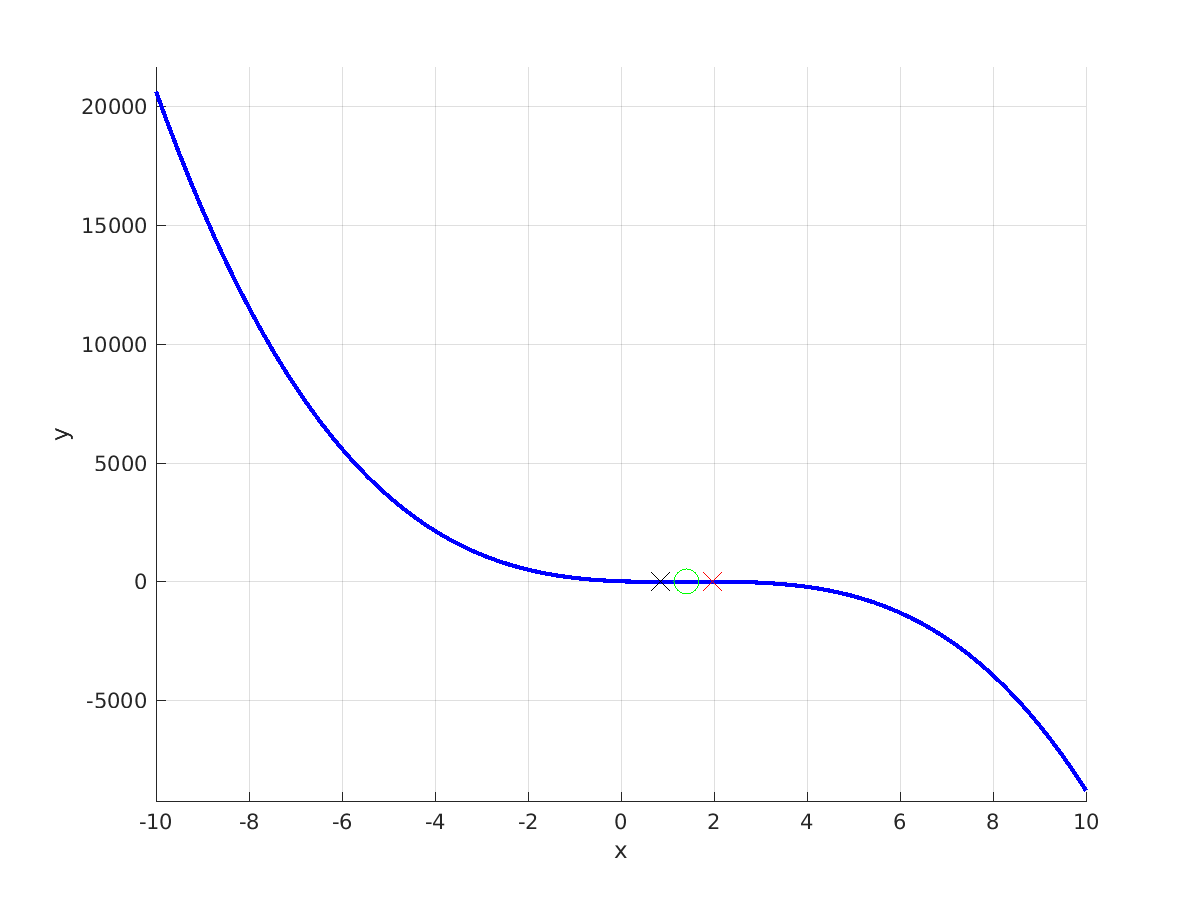
\includegraphics[width=0.8\linewidth]{Abb_zur_Ag_autogenerated_fractions_16.png} \end{center}
  
 \end{enumerate}
 \else\relax\fi
  \end{MAufgabe}